\documentclass{beamer}
\usetheme{Boadilla}
\usepackage{graphicx}
\graphicspath{./Images/}
\title{Predicting NHL Team Points Proposal}
\author{Eric Foote}
\institute{UNBSJ}
\date{September 20th 2018}

\begin{document}
	
	\begin{frame}
		\titlepage
	\end{frame}
	
	\begin{frame}
	"Hockey statistics is in its infancy"\cite{Weissbock} from what started out in the earliest day as a Yahoo group\cite{Vollman} has grown to a few teams having an analytics department that infulences everything from personnal choices to player scouting. (e.g. Toronto)
	\end{frame}
	
	\begin{frame}
	"Over the past few years, though, analytics has been the buzzword around NHL circles. As teams like the Chicago Blackhawks and Los Angeles Kings, winners 
	of four of the past five Stanley Cups, find success through the use of data, other teams will naturally have to follow suit if they want to compete." \cite{Forbes}
	\end{frame}
	
	\begin{frame}
	
	\begin{figure}	
		
\includegraphics[width=0.2\linewidth]{Images/kyle-dubas}
    \end{figure}
	“We felt that Kyle was a hockey man who understood the analytical part of the game,” said Nonis about the hiring of Dubas. “He wasn’t an analyst. To me, there is a pretty big distinction. Kyle understands that these stats and trends are just part of what we do to make decisions. We’re going to use as much as we can going forward.” \cite{Forbes}
	\end{frame}
	
	\begin{frame}
	
	\begin{figure}	
			
\includegraphics[width=0.2\linewidth]{Images/chakya-12-13-620x370}
	\end{figure}
	"Chayka uses analytics as a tool in his decision-making process and as a resource in dealing with players, coaches, agents and opposing GMs." \cite{Chyka}
	"Chayka went on to co-found Stathletes, a hockey analytics company, in 2010 while earning a business degree. Stathletes' goal was to use video analysis to create statistics that better help measure the ability and value of players -- and to make those numbers more accessible." \cite{Chyka}
	\end{frame}
	
	\begin{frame}
	How does this apply to me? \newline
	My project is going to predict the team points 
	\begin{figure}
		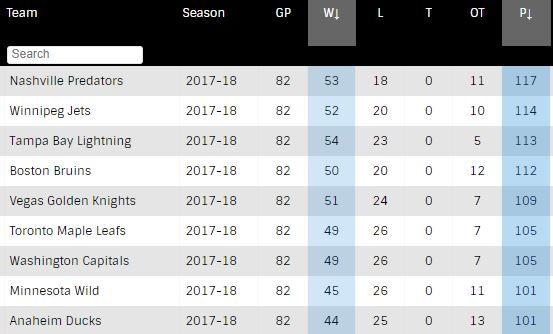
\includegraphics[width=0.7\linewidth]{Images/PicturePoints}
	\end{figure} 	
	\end{frame}

	\begin{frame}
	How does the NHL calculate points? \newline
	A win is 2 points \newline
	A overtime loss or shootout loss is 1 point  \newline
	A loss is no points
	\end{frame}

	\begin{frame}
	There are 31 teams currently in the NHL \newline
	There are 2 confrences the East and West: \newline
	In the 16 team East there is the Atlantic Division and the Metropolitan \newline
	In the 15 team West there is the Central Division and the Pacific \newline
	For the datasets that I am considering there is only going to be 30 teams \newline
	For the predictor year there will be \textbf{31} teams
	\end{frame}

	\begin{frame}
	The teams that I am going to be predicting are:\newline
	Anaheim Ducks \newline
	Boston Bruins \newline
	Buffalo Sabres \newline
	Calgary Flames \newline
	Carolina Hurricanes \newline
	Chicago Blackhawks \newline
	Colorado Avalanche \newline
	Columbus Blue Jackets \newline
	Dallas Stars \newline 
	Detroit Red Wings \newline
	Edmonton Oilers \newline
	Florida Panthers \newline
	Los Angeles Kings \newline
	Minnesota Wild \newline
	Montreal Canadiens \newline
	Nashville Predators \newline 
	New Jersey Devils \newline
	New York Islanders \newline
	\end{frame}

\begin{frame}
	New York Rangers \newline
	Ottawa Senators \newline
	Philadelphia Flyers \newline
	Phoenix Coyotes \newline
	Pittsburgh Penguins \newline
	Saint Louis Blues \newline
	San Jose Sharks \newline
	Tampa Bay Lighting \newline
	Toronto Maple Leafs \newline
	Vancouver Canucks \newline
	\textbf{Vegas Golden Knights} \newline
	Washington Capitals \newline
	Winnipeg Jets
\end{frame}

	\begin{frame}
		\begin{figure}
		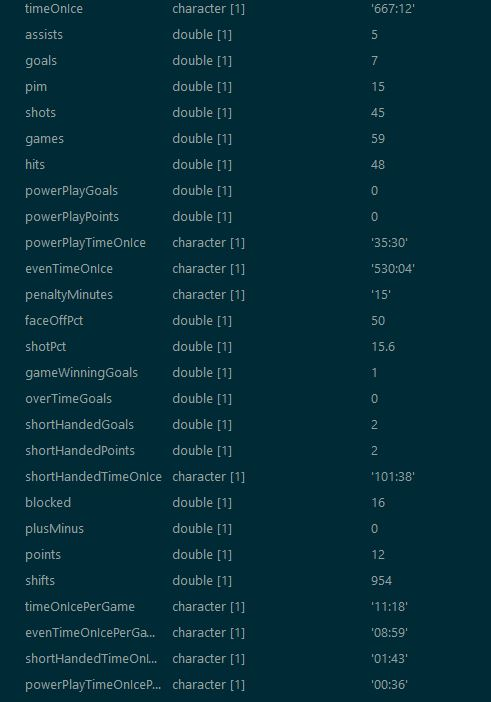
\includegraphics[width=0.5\linewidth]{Images/PlayerCapture}
	\end{figure} 
	\end{frame}

	\begin{frame}
	\begin{figure}
		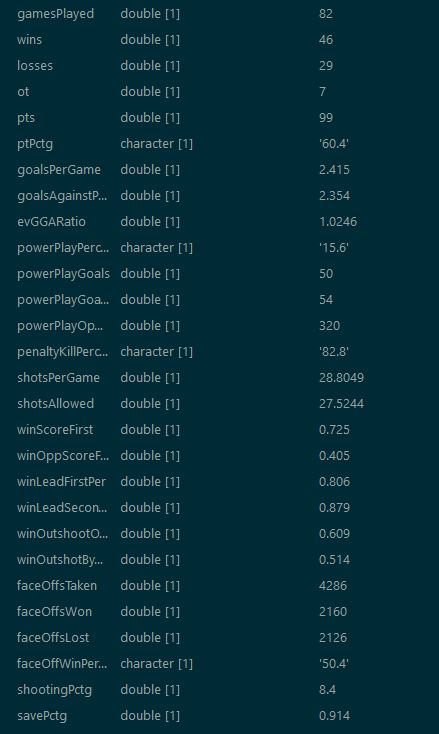
\includegraphics[width=0.4\linewidth]{Images/TeamCapture}
	\end{figure} 
\end{frame}

\begin{frame}
	\begin{figure}
		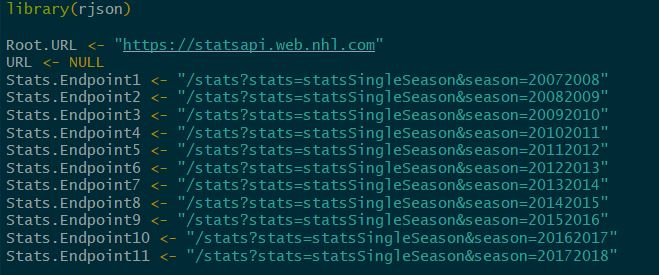
\includegraphics[width=1\linewidth]{Images/Block1}
	\end{figure}
	
\end{frame}

\begin{frame}
\begin{figure}
	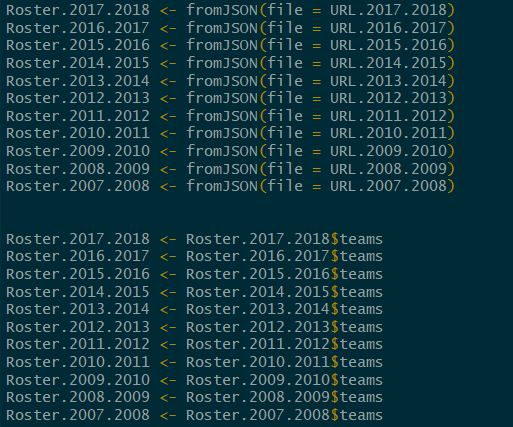
\includegraphics[width=0.7\linewidth]{Images/Block2}
\end{figure}

\end{frame}

\begin{frame}
\begin{figure}
	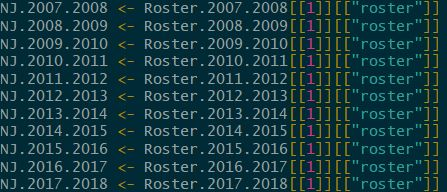
\includegraphics[width=0.7\linewidth]{Images/Block3}
\end{figure}
This block was replicated 30 times \newline
The last line is used once more for Vegas
\end{frame}

\begin{frame}
\begin{figure}
	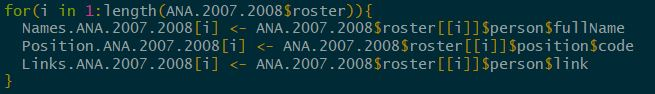
\includegraphics[width=0.7\linewidth]{Images/Block4}
\end{figure}

\end{frame}

\begin{frame}
\begin{figure}
	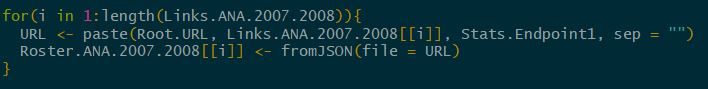
\includegraphics[width=0.7\linewidth]{Images/Block5}
\end{figure}
\begin{figure}
	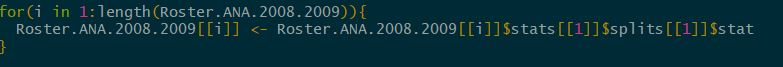
\includegraphics[width=0.7\linewidth]{Images/Block6}
\end{figure}

\end{frame}

\begin{frame}
	\textbf{Methods} \newline
	Linear Regression  \newline
	Logistic Regression  \newline
	Gradient Boosted Decision Trees \newline
	\textit{Other Trees}  If time Permits  
	
\end{frame}

\begin{frame}
	The plan currently is that I am going to use these three different methods to predict team points for the 2017-2018 season using some of these variables from the 2007-2008 to the 2016-2017 seasons. \newline
	
\end{frame}

\begin{frame}
TimeLine:
\begin{center}
	\begin{tabular}{|c |c|}
		\hline
		Item & Rough Week Length \\ 
		\hline
		Sum of Squares & 1 \\
		\hline
		Logistic Regression & 2-3 \\
		\hline
		Gradient Boosted Tree & 2-3 \\
		\hline
		Other Regression Trees & 1-2? \\
		\hline
		Analysis & 1.5 \\
		\hline
		Report Writing & 1.5 \\
		\hline
	\end{tabular}
\end{center}

\end{frame}

\begin{thebibliography}{9}
\bibitem{Weissbock}
Joshua Weissbock Forecasting Success in the
National Hockey League using
In-Game Statistics and Textual Data School of Electrical Engineering and Computer Science
Faculty of Engineering
University of Ottawa,  Ottawa, Canada, 2014
\bibitem{Vollman}
Robert Vollman Aug 24, 2016 \newline http://www.hockeyabstract.com/thoughts/abriefhistoryofhockeyanalyticsconferences
\bibitem{Forbes}
Mark J Burns Sep 25, 2014 \newline https://www.forbes.com/sites/markjburns/2014/09/25/assistant-gm-kyle-dubas-injects-youth-smarts-into-maples-leafs-front-office/684caa5c188e
\bibitem{Chyka}
Josh Cooper October 10 2018 \newline
$http://www.espn.com/nhl/story/_/id/20922909/nhl-arizona-coyotes-gm-john-chayka-more-just-numbers-nerd$
\bibitem{Chyka2}
http://arizonasports.com/story/1346879/coyotes-chayka-happy-home/
\bibitem{Dubas}
https://torontosun.com/sports/hockey/nhl/toronto-maple-leafs/soo-roots-run-deep-for-new-maple-leafs-gm-kyle-dubas

\end{thebibliography}
\end{document}